\chapter{Methodology}
\label{chap:Three}

\section{Capturing video and cutting into frames}
The first step is to 


\section{Face detection}
Face detection was done 

\section{Face Pre-processing}
The faces could not be passed to a neural network as red, green and blue channels 

As shown in figure \ref{figure:Faces} the difference between RGB and LBP images is huge, the LBP highlights more distinct features in the face like the mouth, eyes and edges more than the RGB image does.  After this process the faces distinct feature are much more detectable and the image is ready to be passed to the neural network.
 \par
 \begin{figure}[H]
\centering
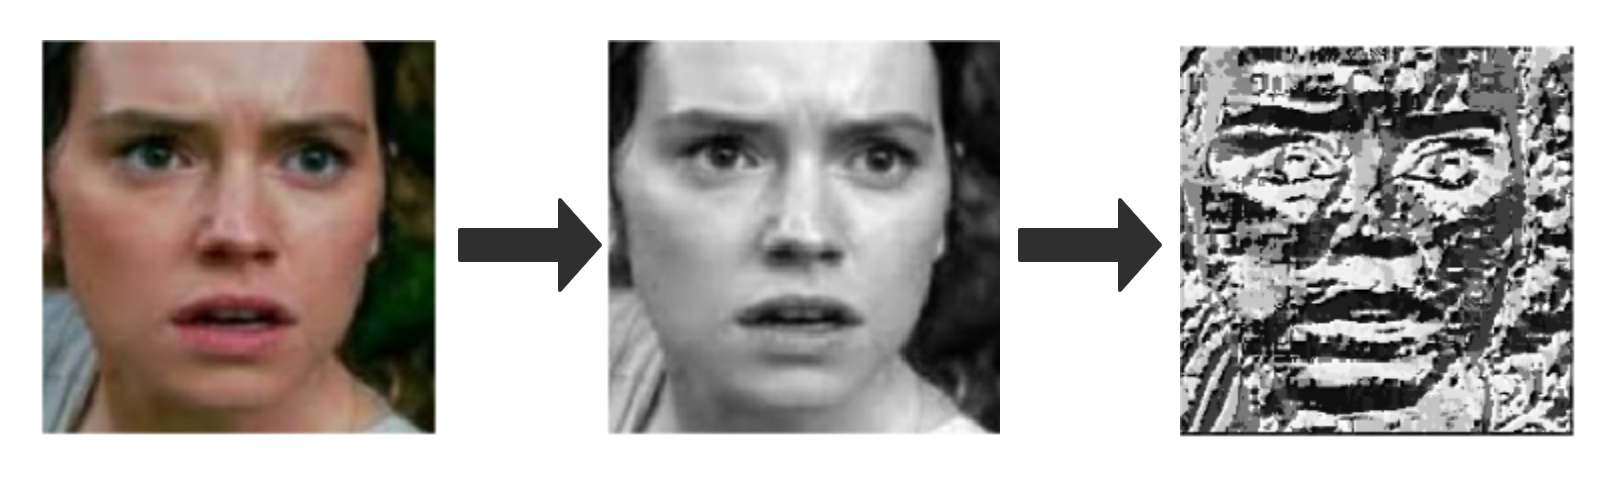
\includegraphics[width=15cm]{Figures/faces.png}
\caption{Conversion from RGB to LBP }
\label{figure:Faces}
\end{figure}

